
\begin{table}[!htbp] \centering
	\section{Lås}
	\label{tab:laas1}
\begin{tabular}{|p{6cm}|p{8cm}|}
	\hline
		\textbf{Løsning}				&Elektrisk karm lås TFS-A21 \\ \hline
		\textbf{Producent} 			&Ukendt \\ \hline
		\textbf{Tilslutning} 		&12V DC - 0.6A \\ \hline
		\textbf{Beskrivelse} 		&Elektrisk karm lås med bevægelig pal \\ \hline
		\textbf{Krav} 				&Skal monteres med slutblæk \\ \hline
		\textbf{Fordele}				& \\ \hline
		\textbf{Ulemper} 			&Slutstykket begrænser montering (udfræsning). Den bevægelige pal skal smøres. \\ \hline
		\textbf{Pris} 				&65 kr \\ \hline
		\textbf{Link} 				&http://goo.gl/SDvjkd \\ \hline	
		\multicolumn{2}{|c|}{
			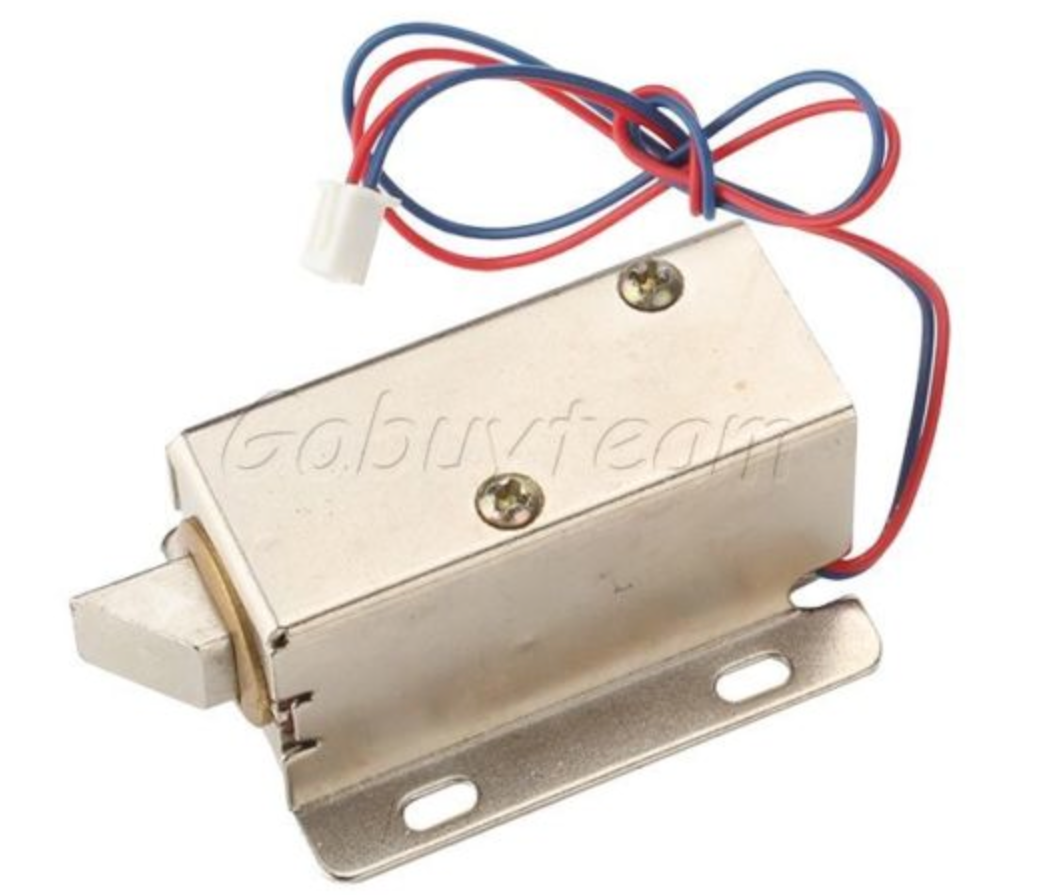
\includegraphics[height=3cm]{billeder/TFS-A21.png}} \\ \hline	
\end{tabular}
\end{table}

\begin{table}[!htbp] \centering
	\label{tab:laas2}
\begin{tabular}{|p{6cm}|p{8cm}|}
	\hline
		\textbf{Løsning}				&Elektromagnetisk lås 60kg \\ \hline
		\textbf{Producent} 			&KingGo \\ \hline
		\textbf{Tilslutning} 		&12 V DC - 0.3A\\ \hline
		\textbf{Beskrivelse} 		&Elektromagnetisk lås uden bevægelige dele \\ \hline
		\textbf{Krav} 				&Skal monteres med metal stykke \\ \hline
		\textbf{Fordele}				&Skal kun skrues fast \\ \hline
		\textbf{Ulemper} 			& \\ \hline
		\textbf{Pris} 				&115 kr \\ \hline
		\textbf{Link} 				&http://goo.gl/ewKYfa\\ \hline	
		\multicolumn{2}{|c|}{ 
			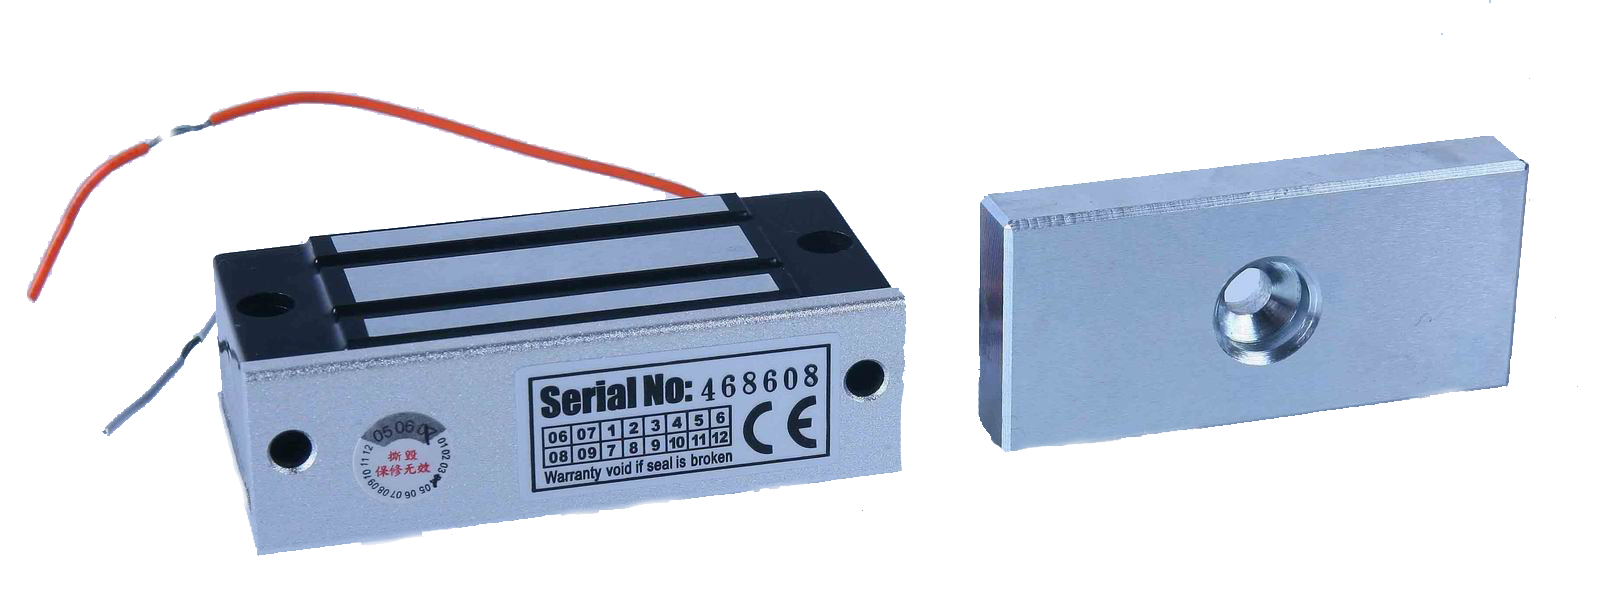
\includegraphics[height=3cm]{billeder/magnetic.png}} \\ \hline	
\end{tabular}
\end{table}

\subsection{Løsning}

Valget et faldet på den elektromagnetiske lås fra KingGo. Denne lås er valg da den er simpel og let at sætte op, da der ikke skal fræses ud for at benytte denne type lås. Ydermere så vil låsen automatisk låse sig fast, hvis modtager pladen er ude for rækkevidde og denne fysisk skubbes hen til elektromagneten. I testmiljøet vil en 12V lyskilde agere lås.